\documentclass[a4paper,12pt]{article}
\usepackage{geometry}
\geometry{a4paper, margin=1in}

\usepackage{amsmath, amssymb}
\newcommand{\rvline}{\hspace*{-\arraycolsep}\vline\hspace*{-\arraycolsep}}
% See https://tex.stackexchange.com/questions/323297/typing-block-matrices-with-zero-blocks-and-separators
\usepackage{tikz}
\usetikzlibrary{quantikz2}

\usepackage{graphicx}
\usepackage{caption}

\usepackage{fancyhdr}
\usepackage{graphicx}
\usepackage{titlesec}
\usepackage{titling}
\usepackage{xcolor}
\usepackage{hyperref}
\hypersetup{
    colorlinks=true,
    linkcolor=blue,
    filecolor=magenta,      
    urlcolor=cyan,
}

% Header and Footer
\pagestyle{fancy}
\fancyhf{}
\fancyhead[L]{
\includegraphics[height=0.8cm]{logo.jpg}} % Include your institution logo
\fancyhead[C]{\footnotesize \textbf{\courseName}}
\fancyhead[R]{
\includegraphics[height=0.8cm]{ionq_logo_simple.png}}

\fancyfoot[L]{\projectName}
\fancyfoot[C]{Page \thepage}
\fancyfoot[R]{\today}

% Title formatting
\pretitle{\begin{center}\LARGE \bfseries}
\posttitle{\end{center}\vspace{0.5cm}}
\preauthor{\begin{center}\normalsize}
\postauthor{\end{center}}
\predate{\begin{center}\small}
\postdate{\end{center}\vspace{1cm}}

% Section formatting
\titleformat{\section}[block]{\Large\bfseries}{\thesection}{1em}{}
\titleformat{\subsection}[block]{\large\bfseries}{\thesubsection}{1em}{}
\titleformat{\subsubsection}[block]{\bfseries}{\thesubsubsection}{1em}{}

% Custom commands for student details
%\newcommand{\studentName}{Hyunseong Kim}
%\newcommand{\studentID}{20195048}
\newcommand{\courseName}{2024 IonQ summer Mentoring}
%\newcommand{\courseCode}{MM4020}
\newcommand{\assignmentTitle}{OptTrot}
%\newcommand{\dueDate}{June 30, 2024}

\newcommand{\projectName}{OptTrot}

\newtheorem{theorem}{Theorem}
\newtheorem{lemma}{Lemma}
\newtheorem{corollary}{Corollary}
\newtheorem{definition}{Definition}
\newtheorem{observation}{Observation}


\begin{document}

% Title Section
\begin{center}
%    %
\includegraphics[width=0.15\textwidth]{logo.png}\par\vspace{1cm} % Include your institution logo
%    {\scshape \courseName \par}
%    {Final Assignment \par}
%    \vspace{0.5cm}

    \vspace{0.5cm}
    {\Large\bfseries \assignmentTitle \par}
    {\large Optimized Trotter Circuit Library \par}
    \vspace{1cm}
    {
    \noindent
    Hyunseong Kim

    GIST, qwqwhsnote@gm.gist.ac.kr
    \vspace{0.5cm}

    \begin{minipage}{0.45\textwidth}
        \centering
        \textbf{Memebers}

        Hyunseong Kim

        Hanseo Kim
        
        Gaya Yun
    \end{minipage}
    \begin{minipage}{0.45\textwidth}
        \centering
        \textbf{Mentor}

        Sayonee Ray
    \end{minipage}
    }
%    {\itshape \studentName \par}
%    {Student ID: \studentID \par}
%    \vspace{0.5cm}
%    {\large \today \par}
    \begin{abstract}
        OptTrot is a library of generating optimized Trotter circuit for a given hamiltonian.
        Trotterization is a standard way to accomplish time evolution circuit on gate model
        computer, however, their long depth circuit has significantly contributed to 
        the hurdle of practical application.
        In the library, we combined commuting partition method and Pauli Frame search method.
        If the given Pauli term mutually commuted with Pauli Frame axis, then the Clifford gate
        combination was reduced to combinations of CX gate. 
        Moreover, their specific decomposition
        is easily derived from Gauss elimination of matrix over module 2 field, $\mathbb{Z}/2 \mathbb{Z}$.
        In the library, the overall process are easily achieved by convenience interfaces.
        Furthermore, researchers could combine the library with various optimization tools from classic 
        to quantum methods for partitioning of Pauli terms.
    \end{abstract}
\end{center}


%\tableofcontents
%wpage

\section{Introduction}

Aim of the report is to introduce about theoretical backgrounds of
OptTrot library. Why the library was developed, and how we can optimize 
the circuit for time evolution with Trotterization method.
In OptTrot, many optimization techniques were used to design and implement
the library. Each 

Trotterization is a standard method used to implement a time evolution operator 
by combining several local hamiltonian evolution operators.
By using the method, we can expect the approximated operator closed to the original
operator, even the local terms did not commute with each other with quadratic, $O(t^2)$, error,
and better bounds with higher order approximations\cite{suzuki_finding_2005}.

\begin{equation}
    \lim_{n \rightarrow \infty} (e^{A/2} e^{B/2})^n = e^{A+B}
\end{equation}

However, standard Trotterization method increases circuit depth with linear order 
by number of Pauli terms. That is, a hamiltonian whose number of local terms are $N$
has, at least, $N$ time deeper circuit than single Pauli term evolution circuit.
If the time evolution was an ultimate goal to achieve in quantum circuit, 
it could be meaningful, but in the most algorithms and applications, time evolution 
is just a part of the whole process. 
Thus, reducing techniques are significant to apply the quantum computer to general applications.
In addition, increased circuit depth for reducing Trotter error yields 
impractical errors on NISQ, which caused by gate fidelity between ideal and implemented gates.
By the limitation, there have been studied many alternative methods, to implement a time evolution operator 
with shorter depth circuit than Trotterization, 
such as linear combination of unitary(LCU) method\cite{dewolf2023quantumcomputinglecturenotes}, Qubitization\cite{Low_2019}, 
Taylorization\cite{PhysRevLett.114.090502}, and Fractional query\cite{Berry_2014}.
Such methods make the evolution circuit more practical, however, they loose 
identity of the given system, especially the cases, when the given hamiltonian is nearly commute
or local observable was a dominant feature\cite{childs_theory_2021}. 
Only problem is a high cost of the Trotterization circuit. 
However, there is an unwarranted problem of Trotterization. 
A problem is circuit synthesis process of standard method\cite{nielsen2010quantum}
is often misinterpreted as a problem of Trotterization.

\begin{figure}[!ht]
    \centering
    \begin{quantikz}
    & \gate{H} & \ctrl{1} & & \ctrl{1} & \gate{H} & \\
    &          & \targ{} & \gate{RZ}& \targ{} & & \\
    \end{quantikz}
    \label{fig:trotter_standard_circuit}
    \caption{Example of trotter evolution circuit. Where $H = X \otimes Z$}
\end{figure}

How can we optimize the circuit synthesis for trotter evolution circuit?
There have been various studies of circuit optimization\cite{johann_2023, PhysRevResearch.5.023146}
but in here, the report is focusing especially for trotter circuit implementation. 

Schmitz et al would be a milestone paper\cite{schmitz_graph_2023} for the implementation.
They analyzed what term would be rotated when we apply entanglement gates 
on quantum circuit using Pauli Frame, and suggested a practical method to find a better depth
evolution circuit of given hamiltonian. 
However, the paper has some limitations in frame search methods,
which is not practical for rapidly generating various hamiltonian circuits.
In the library, we combine the tools with commuting partitioning method.
Especially, we will focus on an attempt that author Kim's study\cite{hyunseong_2023_8434890}, 
using commuting pair to reduce the circuit depth. 

This report consist of 3 parts,

\begin{enumerate}
    \item Commuting partition effect on Trotter error.
    \item Pauli Frame method and their limitation.
    \item Pauli Frame method on mutually commuting partition. 
    \item Construction of mutually commuting partition.
\end{enumerate}

\section{Commuting Partition for Optimization}

When hamiltonian is given, first thing to do 
is decomposing into combination of Pauli elements.

\begin{equation}
    H \rightarrow \sum_i \lambda_i P_i
\end{equation}

The decomposed Pauli terms are used for not only time-evolution
but also measurement of the hamiltonian.
In circuit optimization, the commuting partition 
provides more convenience properties for manipulation.

\subsection{Trotter Error by applying order}

It is well known that the exponential mapping error is represented with Baker Campbell Hausdorff formula.
Usually, the formula is not written with commutator form, Childs et al proved that the error term 
as a function of sequential commutator of local terms\cite{childs_theory_2021}.

\begin{equation}
    O(\alpha t^2)
\end{equation}

The result theorem of Childs et al allow us to calculate 
the error boundary more precisely including a physical structure 
of the given hamiltonian.
Furthermore, the applying order effect of $\exp(-it H_l), H = \sum_L H_l$ 
is well derived from the theorem.

\begin{theorem}
    Let $H = \sum_i^N H_i$ be an operator consisting of $N$ sum of local hmailtonian,
    and $t\geq 0$.
    Let $S(t) = \Pi_{k=1}^M \Pi_{l=1}^N \exp(t a_{kl} H_{\pi_k(l)})$ be a $p$-th order
    Suzuki Trotter formula, then it's error term is asymptotically bounded by
    \begin{equation}
        O(\alpha_{com} t^{p+1} \exp(4t M \sum_{l=1}^N || H_l||))
    \end{equation}
    where, $\alpha_{com} = \sum_{l_1, l_2, \dots , l_{p+1}}^N || [H_{l_{p+1}}, \cdots [H_{l_2}, H_{l_1}]]||$
\end{theorem}

For example, let a given hamiltonian was $H = c_i P_i + c_j P_j$.

\begin{equation}
    \exp(-it (c_i) P_i) \exp(-it (c_j) P_j) = \exp(- it (c_i P_i + c_j P_j)) + O (\alpha_{com}t^2)
\end{equation}

then, the leading coefficient becomes $\alpha_{com} = \begin{cases}
    c_i + c_j & \mbox{ if } [P_i, P_j] = 0 \\
    c_i - c_j & \mbox{ if } [P_i, P_j] \neq 0 \\
\end{cases}$.

It is affected by coefficients, their size, and sign, and commutation property.
In the above example, we cannot observe the commutation and anti-commutation
effect, since, if they were commuting to each other, the $O(\alpha_{com} t^2) = 0$.
Let us expand the system to more general case.
Suppose that the given hamiltonian has two representations,

\begin{align}
    H = H_1 + H_2 + H_3  \\
    H =  c_1 P_1 + c_2 P_2 + c_3 P_3 + c_4 P_4 + c_5 P_5\\
    H_1 = c_1 P_1 + c_3 P_3 \\
    H_2 = c_2 P_2\\
    H_3 = c_4 P_4 + c_5 P_5
\end{align}

where, $[H_i, H_j] \neq 0,$ and 
$[P_k, P_l] \neq 0$ if $P_k \in H_i, P_l \in H_j, i \neq j$.

\begin{align}
    \Pi_{l=1}^5 \exp(- i t (c_l P_l)) = \exp(-it H) + O(\alpha_{com 1} t^2)\label{eq:pauli_evolve}\\
    \Pi_{k=1}^3 \exp(- i t (H_k)) = \exp(-it H) + O(\alpha_{com 2} t^2) \label{eq:evolve_commute}
\end{align}

Following the $q=1$ order expansion, then in the first order, the bound error 
coefficients are reduced to 

\begin{align}
    \alpha_{com1} = 2(|| c_1 c_2 [P_1, P_2]|| + || c_1 c_4 [P_1, P_4]|| + || c_1 c_5 [P_1, P_5]||& \\
    + || c_2 c_3 [P_2, P_3]|| + || c_2 c_4 [P_2, P_4]|| + || c_2 c_5 [P_2, P_5]||& \\
    + || c_3 c_4 [P_3, P_4]|| + || c_3 c_5 [P_3, P_5]||)&\\
    \alpha_{com2} = 2(|| [H_1, H_2]|| + || [H_1, H_3]|| + || [H_2, H_3]||)& 
\end{align}


\begin{align}
    0.5 \alpha_{com1} &= ||c_1 c_2|| + ||c_3 c_2|| + ||c_1 c_4|| + ||c_2 c_4|| + ||c_1 c_5|| + ||c_2 c_5||  + ||c_2 c_4|| + ||c_2 c_5||\\
    0.5 \alpha_{com2} &= ||c_1 c_2 + c_3 c_2|| + ||c_1 c_4 + c_2 c_4 + c_1 c_5 + c_2 c_5||  + ||c_2 c_4 + c_2 c_5||
\end{align}


Therefore, by the distribution of $\{c_i\}$ and commutation relationship of the local terms,
the constructed error rate vary.
However, Eq(\ref{eq:evolve_commute}) is just a re-ordering of Eq(\ref{eq:pauli_evolve}), since 

\begin{align}
    \exp(- i t (H_1)) &= \exp(- i t (c_1 P_1)) \exp(- i t (c_3 P_3)) \\ 
    \exp(- i t (H_2)) &= \exp(- i t (c_2 P_2))\\
    \exp(- i t (H_3)) &= \exp(- i t (c_4 P_4)) \exp(- i t (c_5 P_5)) \\ 
\end{align}

This is not at all, local hamiltonian consists of mutually commuting Pauli terms provides us a lot of freedom
to optimize the circuit. 
Whatever we switch and reorder the Pauli terms in the applying trotter circuit,
if the larger structure, $\exp(-it H_j) = \Pi_k \exp(-it c_jk P_jk)$, was preserved then, 
the trotter error would be bounded while we reduce the number of gates in the implementation.
Thus, we don't have to choose one between trotter error and large gate error
to optimize the evolution circuit.

\textbf{Note}: The partitioning the hamiltonian into large local terms does not yield the optimized 
order in every situation. 
The term $\alpha$ only indicates upper bound of the error. So, the minimum trotter error could be 
worse than the arbitrary applying case. 
In here, the main focus is reducing errors associated with gate operations by using minimum number of gates.
See, Fig \ref{fig:evolve_error}.

\begin{figure}
        \centering
        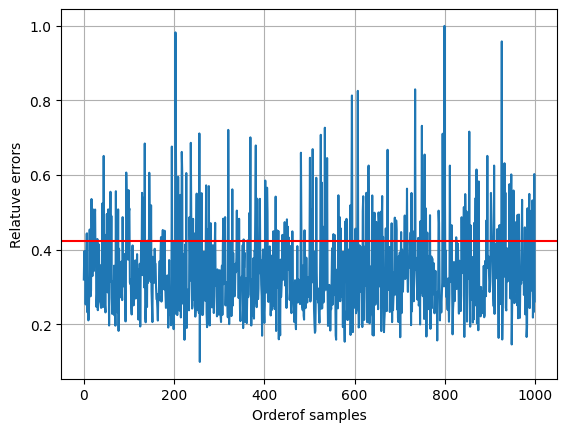
\includegraphics[width=0.8\textwidth]{figures/error rates.png}
        \caption{
            Relative error rate of random Hamiltonian, $H$. 
            The red horizontal line is a largest local hamiltonian decomposition and the each sample are random order of $\exp(-i t P_l)$.
            }
            \label{fig:evolve_error}
\end{figure}

\section{Optimizing a circuit with commuting pairs}

\subsection{Pauli Frame method}

One method to optimize the Trotter circuit is using \textit{Pauli Frame}\cite{schmitz_graph_2023}.
Pauli Frame is a collection of Pauli terms indicating axes on each quantum circuit wires
when we apply Rotation Z gate on the circuit.

\begin{figure}
    \centering
    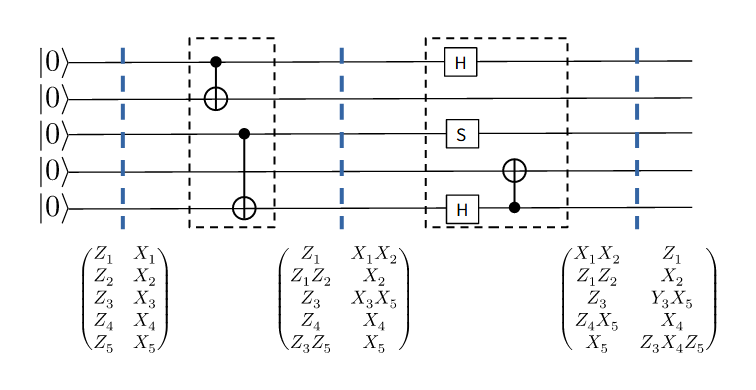
\includegraphics[width = 0.95\textwidth]{figures/Pauli Frame.png}
    \caption{
        Example of Pauli Frame analysis of a quantum circuit. 
        The dashed blue lines are corresponded to the below Pauli Frame.
        If we apply RZ gate on 5th qubit after we applied two CX gates,
        then the rotation gate is corresponding to $\exp(-i t Z_3Z_5)$.
    }
    \label{fig:Pauli Frame}
\end{figure}

Using the method, we can chase what Pauli elements were applied, 
and what elements we can rotate on the circuit.


The original paper formulated the problem as 
Traversal purchaser problem(TPP)\cite{schmitz_graph_2023}.
However, they did not solve the TPP problem and 
used a dynamic programming method to find a proper frame path.
In other word, they manually searched all possible routine
for the given hamiltonian.
There are two major reasons.
To calculate a distance between two frames, $B_i, B_j$, we have to know
all Frame information before we calculate.
However, what frame would be sufficient to represent a trotter path 
for the hamiltonian composites with entanglement gates?.
We cannot know the solution of such problem when arbitrary hamiltonian was given.
The only thing we have is a set of Pauli elements given by the hamiltonian.
Moreover, when two frames were given, what Clifford gates would yield the 
transformation from $B_i$ to $B_j$?.
There is no solid frameworks to make the transformation.
The questions are remained from Schmitz et al paper.

In here, if we found that the route finding algorithm
when the given Pauli elements are mutually commuting to each other.

\subsection{Path search over commuting cliques}

\subsection{Symplectic representation of Pauli elements}

It is natural that the Pauli group is a kind of Clifford group of $Cl_{2,0}$,
where two elements coud generate all elements.

\subsubsection{IZ family}

$I, Z$ family would be a good example to see the process of gate construction
over mutually commuting Pauli set.
Consider that the local term of the hamiltonian are composite of $I, Z$ tensor product.
Then, for a given frame $B$ and suppose that we have to make next frame to have $P = IIZZ$.
Since, we don't have to consider terms containing $X, Y$, we can simply write the term 
as single stabilizer of the Frame, and the required entanglement gate is $CX$ gate only.

\begin{equation}
    B = \begin{bmatrix}
        ZZZI\\
        ZZIZ\\
        ZIZZ\\
        IZZZ
    \end{bmatrix}
    \rightarrow B' = \begin{bmatrix}
        \dots\\
        IIZZ\\
        \dots\\
        \dots
    \end{bmatrix}
\end{equation}

The answer is shortly applying a $CX$ gate on line 1 and 2.

Now, let the representation as binary vector
\begin{equation}
B = \begin{bmatrix}
    ZZZI\\
    ZZIZ\\
    ZIZZ\\
    IZZZ
\end{bmatrix} = \begin{bmatrix}
    1110\\
    1101\\
    1011\\
    0111
\end{bmatrix} = 
\begin{bmatrix}
    \vec{w}_1\\
    \vec{w}_2\\
    \vec{w}_3\\
    \vec{w}_4
\end{bmatrix}
\end{equation}

With the binary represent, 
the CX combination of $i, j$-th wires is identical to generate XOR of two $w_i$s, 
$w_i \oplus w_j$.
XOR is commutative so that, the problem becomes the next statement.

\begin{quotation}
    Find the minimum size subset $\{w_k\} \subset B$ whose XOR products is $P$
    where,

    \begin{equation*}
        P = \oplus_{k} \vec{w}_k 
    \end{equation*}

\end{quotation}

More simply, it is equivalent with finding a binary vector $\vec{x} \in \{0, 1\}^N$ of 

\begin{equation}
    P = \oplus_{i=1}^N x_i \& \vec{w}_i
\end{equation}

The solution could be derived with simple linear algebra on specific field, $\mathbb{Z}/2\mathbb{Z}$.
Logical \textit{XOR}, and \textit{AND} operators form commuting field, $(\mathbb{Z}/2\mathbb{Z} ,\wedge , \&)$.
See the proof in Appendix \ref{appendix:modulo_field}. 
The Gauss elimination process yields a solution of the above problem.

Suppose that we have circuit of the state where the Pauli Frame representation was,

\begin{equation}
    B_i = \begin{pmatrix}
        w_1 &, \cdot \\
        w_2 &, \cdot \\
        w_3 &, \cdot \\
        w_4 &, \cdot \\
    \end{pmatrix},
    \,
    \begin{matrix}
        w_1 &= Z_2Z_3Z_4 &= ZZZI &= 1110_{sym}\\
        w_2 &= Z_1Z_3Z_4 &= ZZIZ &= 1101_{sym}\\
        w_3 &= Z_1Z_2Z_4 &= ZIZZ &= 1011_{sym}\\
        w_4 &= Z_1Z_2Z_3 &= IZZZ &= 0111_{sym}\\
    \end{matrix}
\end{equation}

and we want to apply $\exp(-i t Z1Z2)$ gate on circuit, what CX gate combination yieds
the quantum circuit state for the unitary operator, by simply applying RZ gate on a wire?
Luckily, XOR is commute as like the CX gate becomes a conjugation of itself.
Let, $v =[1, 1, 0, 0]^T$, it is a symplectic representation of $Z_1Z_2$,
and $x = [x_1, x_2, x_3, x_4]^T, x_i \in \{0, 1\}$. 

\begin{equation}
    M x = v
\end{equation}

\begin{equation}
    M = \begin{bmatrix}
            & \rvline &     & \rvline &      & \rvline &  \\
        w_1 & \rvline &  w_2& \rvline &  w_3 & \rvline &  w_4\\
            & \rvline &     & \rvline &      & \rvline &  \\
    \end{bmatrix}
\end{equation}

\begin{equation} 
    \begin{bmatrix}
        0 & 1 & 1 & 1 \\
        1 & 0 & 1 & 1 \\
        1 & 1 & 0 & 1 \\
        1 & 1 & 1 & 0 \\
\end{bmatrix} \cdot \begin{bmatrix}
        x_1 \\
        x_2 \\
        x_3 \\
        x_4 \\
    \end{bmatrix} 
    = 
    \begin{bmatrix}
        1 \\
        1 \\
        0 \\
        0 \\
    \end{bmatrix}
\end{equation}

With Gauss elimination method, Reduced row echelon form would be obtained.

\begin{eqnarray}
    \begin{bmatrix}
        M &\rvline& v\\
    \end{bmatrix} \rightarrow 
    \begin{bmatrix}
        1 & 1 & 0 & 0 & \rvline & 0\\
        0 & 1 & 1 & 0 & \rvline & 1\\
        0 & 0 & 1 & 0 & \rvline & 0\\
        0 & 0 & 0 & 1 & \rvline & 0\\
    \end{bmatrix}
\end{eqnarray}


\begin{enumerate}
    \item $w_1 \oplus w_2 = 0$
    \item $w_2 \oplus w_3 = 1$
    \item $w_3 = 0$
    \item $w_4 = 0$
\end{enumerate}

Thus, we get $x = [1, 1, 0, 0]$, and


\begin{equation}
    [0, 1, 1, 1] \oplus [1, 0, 1, 1] = [1, 1, 0, 0]
\end{equation}

It means that CX over 1st and 2nd yields $Z1Z2 = IIZZ$ Pauli element on the frame.
The process reached the same point we had predicted at first.


\begin{center}
    \begin{quantikz}
        & \slice[rotate=90]{$B_1$}   & \ctrl{1}  & \slice{$B_2$}&\\
        &                   & \targ{}   &                &\\
        &                   &           &                &\\
        &                   &           &                &
    \end{quantikz}
\end{center}

\begin{equation}
    B_i = \begin{pmatrix}
        ZZZI & \cdot \\
        ZZIZ & \cdot \\
        ZIZZ & \cdot \\
        IZZZ & \cdot \\
    \end{pmatrix}
    \rightarrow_{CX (1, 2)}
    B_{i+1} = \begin{pmatrix}
        ZZZI & \cdot \\
        \mathbf{IIZZ} & \cdot \\
        ZIZZ & \cdot \\
        IZZZ & \cdot \\
    \end{pmatrix}
\end{equation}

The above process holds same for $X$ and $Y$ families each.
Gauss elimination process is enough to determine the exact entanglement
mapping.
However, we cannot adopt the process to the general local terms.
Since, there is no guarantee that the CX gate is enough to 
contruct Clifford gate that connects two given frames.
Rhere are 5 number of entanglements gate to make 
a Pauli terms from one frame to the other frame\cite{schmitz_graph_2023}.

\begin{center}
    \begin{quantikz}
        &\ctrl{1}& \ctrl{1}      &\ctrl{1}     &\\
        &\targ{} & \phase{}    &\push{\odot} &
    \end{quantikz}

    \begin{quantikz}
        &\targ{1}\wire[d][1]{a}& \targ{1}\wire[d][1]{a}&\\
        &\targ{} & \push{\odot}  &
    \end{quantikz}

    \begin{quantikz}
        &\push{\odot} \wire[d][1]{a}&\\
        &\push{\odot} & 
    \end{quantikz}
\end{center}


However, if they were mutually commuting to each other,
the above process could be applied to find a frame path in the commuting set.

\subsection{General Commuting set}

\begin{theorem}
In $N$ qubit system, for a given Pauli term, $p$, and Pauli frame, $B$,
if $p$ is commute with all terms in stabilizers of $B$, $\{s_i\}_{i=1}^N$,
then a frame $B'$ where $p \in \mbox{Stab}(B')$ is derived 
from $B$ at most $N-1$ number of CX gates.

\begin{equation}
    B_0 \rightarrow B'
\end{equation}
\end{theorem}
%the maximum size of mutually commuting Pauli subgroup, $P$, is $2^N$.
%Let $G \subset P$ be a generator of $P$ where, $\forall p \in P, \exists \{g_i\} \subset G$
%such that, $p = \wedge_i g_i$.
%Then, any set of Pauli elements on Frame 
%\end{theorem}

To prove the theorem, we need next theorems\cite{sarkar_sets_2021} about 
commuting subsets of Pauli group on $N$ qubits system.

\begin{theorem}
    For $N$ qubits system, generalized Pauli group, $\mathcal{P}/K$, on the space satisfies the next,

    \begin{itemize}
        \item A cardinality of maximally commuting subset of $\mathcal{P}/K$ is $2^N$.
        \item A maximally commuting subset be a subgroup.
        \item For subgroup $S \subset \mathcal{P}/K, |S| = 2^l$, it's generating set $G$ always exists and $|G| \geq l$.
    \end{itemize}
\end{theorem}


\begin{lemma}
    For a given generating set $G$ of mutually commuting subgroup in $\mathcal{P}/K$, so that $|G| = N$, 
    if a Pauli element, $p$, is mutually commuting with $G$,
    then $p \in \langle G \rangle$.
\end{lemma}

\textbf{Proof}:
If $p \in G$, it is done. Let $p \notin G$.
Suppose $p \notin <G>$, then there is a element $g\in <G>$ such that
$[p, g] \neq 0$. However, $g = n_1 g_1 \cdot n_2 g_2 \cdot \dots \cdot n_N g_N$, and 
$[p, g_i] = 0, \forall i \in [N]$.
In addition, $[p, g_i g_j] =0$ if $[p, g_i] =0$ and $[p, g_j]=0$.
Thus, $[p, n_1 g_1 \cdot n_2 g_2 \cdots \dots \cdots n_N g_N] =0, \!$.
Therefore, $p \in \langle G \rangle$.

\begin{corollary}
    For given two frames, $B_i, B_j$, if their stabilizers are mutually commuting,
    \begin{enumerate}
        \item They are minimum generating sets each for mutually commuting subgroup of $N$ qubit Pauli group.
        \item $\langle \mbox{Stab}(B_i)\rangle = \langle \mbox{Stab}(B_j)\rangle$
        \item These two frames are connected with a combination of CX gates.
    \end{enumerate}
\end{corollary}

\textbf{Proof}: 
By the lemma, all Pauli element in $\mbox{Stab}(B_j)$ are in $\langle \mbox{Stab}{B_i} \rangle$.
So do, $\forall p \in \langle \mbox{Stab}(B_j)\rangle, p \in \langle \mbox{Stab}(B_i)\rangle$, and vice verse. 


The above theorems guarantees that we can build Clifford operator 
with only a combination of CX gates. 
In the end, the exact route to get each term in the stabilizer of $B_2$


\subsection{Summary of Clifford operator search process}

Condition: For given two frames, $B_1, B_2$, $\lambda(\mbox{Stab}(B_1), \mbox{Stab}(B_1)) = 0$

\begin{enumerate}
    \item Calculate the $\oplus, \mbox{Stab}(B_1)$ representation of $p$, $\forall p \in \mbox{Stab}(B_2)$, using RRE over $\mathbb{Z}/2 \mathbb{Z}$.
    \item 
\end{enumerate}



\section{Mutually Commuting Partition}

The remained question is how can we construct mutually commuting partition, 
from the given hamiltonian and its Pauli polynomial representation.
The answer is \textit{we cannot do that efficiently on classical computer}.
Suppose that we constructed a graph that indicates commuting relationship
of all Pauli terms in the hamiltonian. See Fig %\ref{}.

Partitioning the given Pauli elements is equivalent with \textit{Max-clique}
problem in computer science and it is a well-known NP-hard problem\cite{karp_reducibility_1972}.

There are practical algorithms in many graph libraries.%#\cite{} Networkx, Graph-tools, Rustworkx et cetra.
 In addition, many quantum computer companies provide convenience interfaces for clique problems. 
%D-Wave\cite{} 
%QuEra\cite{}
Despite the

\subsection{Solve clique problem on Quantum computer}

Kurita et al, 
They also investigated an algorithm to find max-clique with limited size clique solver
which is smaller than the given problem.

Which method is the most efficient method for the problem? 
Well, the answer is we don't know yet. 
Sometimes quantum algorithm would show better with QAOA or annealing system,
but by the situation classic method could have some advantages.
Choosing an algorithm is a job of researchers or users who want to generate optimized 
Trotter circuit. In here, providing a convenience interface would be enough.

%\section{Conclusion}
%
%In the report, we overlook the trotter error affected by order and hamiltonian structure 
%in $n$-th order Suzukit-Trotter formula.

\appendix

\section{Proof of Modulo field}
\label{appendix:modulo_field}

$(\mathbb{Z}/2\mathbb{Z} ,\wedge , \&)$.

Denote, XOR($\wedge$) as $\oplus$ and, AND($\&$) as $\odot$,

\begin{equation}
    \begin{matrix}
        0 \oplus 0 & = &0\\
        0 \oplus 1 & = &1\\
        1 \oplus 0 & = &1\\
        1 \oplus 1 & = &0\\
    \end{matrix}
    \, 
    \begin{matrix}
        0 \odot 0 & = &0\\
        0 \odot 1 & = &0\\
        1 \odot 0 & = &0\\
        1 \odot 1 & = &1\\
    \end{matrix}
\end{equation}

Addition 

\begin{enumerate}
    \item a
\end{enumerate}

%Bibliography
\bibliographystyle{unsrt}  
\bibliography{references}  

\end{document}
